\documentclass[aspectratio=169]{../latex_main/tntbeamer}  % you can pass all options of the beamer class, e.g., 'handout' or 'aspectratio=43'
\usepackage{dsfont}
\usepackage{bm}
\usepackage[english]{babel}
\usepackage[T1]{fontenc}
%\usepackage[utf8]{inputenc}
\usepackage{graphicx}
\graphicspath{ {./figures/} }
\usepackage{algorithm}
\usepackage[ruled,vlined,algo2e,linesnumbered]{algorithm2e}
\usepackage{hyperref}
\usepackage{booktabs}
\usepackage{mathtools}

\usepackage{amsmath,amssymb}

\DeclareMathOperator*{\argmax}{arg\,max}
\DeclareMathOperator*{\argmin}{arg\,min}

\usepackage{amsbsy}
\newcommand{\vect}[1]{\bm{#1}}
%\newcommand{\vect}[1]{\boldsymbol{#1}}

\usepackage{pgfplots}
\pgfplotsset{compat=1.16}
\usepackage{tikz}
\usetikzlibrary{trees} 
\usetikzlibrary{shapes.geometric}
\usetikzlibrary{positioning,shapes,shadows,arrows,calc,mindmap}
\usetikzlibrary{positioning,fadings,through}
\usetikzlibrary{decorations.pathreplacing}
\usetikzlibrary{intersections}
\pgfdeclarelayer{background}
\pgfdeclarelayer{foreground}
\pgfsetlayers{background,main,foreground}
\tikzstyle{activity}=[rectangle, draw=black, rounded corners, text centered, text width=8em]
\tikzstyle{data}=[rectangle, draw=black, text centered, text width=8em]
\tikzstyle{myarrow}=[->, thick, draw=black]

% Define the layers to draw the diagram
\pgfdeclarelayer{background}
\pgfdeclarelayer{foreground}
\pgfsetlayers{background,main,foreground}

% Requires XeLaTeX or LuaLaTeX
%\usepackage{unicode-math}

\usepackage{fontspec}
%\setsansfont{Arial}
\setsansfont{RotisSansSerifStd}[ 
Path=../latex_main/fonts/,
Extension = .otf,
UprightFont = *-Regular,  % or *-Light
BoldFont = *-ExtraBold,  % or *-Bold
ItalicFont = *-Italic
]
\setmonofont{Cascadia Mono}[
Scale=0.8
]

% scale factor adapted; mathrm font added (Benjamin Spitschan @TNT, 2021-06-01)
%\setmathfont[Scale=1.05]{Libertinus Math}
%\setmathrm[Scale=1.05]{Libertinus Math}

% other available math fonts are (not exhaustive)
% Latin Modern Math
% XITS Math
% Libertinus Math
% Asana Math
% Fira Math
% TeX Gyre Pagella Math
% TeX Gyre Bonum Math
% TeX Gyre Schola Math
% TeX Gyre Termes Math

% Literature References
\newcommand{\lit}[2]{\href{#2}{\footnotesize\color{black!60}[#1]}}

%%% Beamer Customization
%----------------------------------------------------------------------
% (Don't) Show sections in frame header. Options: 'sections', 'sections light', empty
\setbeamertemplate{headline}{empty}

% Add header logo for normal frames
\setheaderimage{
	% 
\includegraphics[height=\logoheight]{figures/TNT_darkv4.pdf}
	
\includegraphics[height=\logoheight]{../latex_main/figures/luh_logo_rgb_0_80_155.pdf}
	% 
\includegraphics[height=\logoheight]{figures/logo_tntluh.pdf}
}

% Header logo for title page
\settitleheaderimage{
	% 
\includegraphics[height=\logoheight]{figures/TNT_darkv4.pdf}
	
\includegraphics[height=\logoheight]{../latex_main/figures/luh_logo_rgb_0_80_155.pdf}
	% 
\includegraphics[height=\logoheight]{figures/logo_tntluh.pdf}
}

% Title page: tntdefault 
\setbeamertemplate{title page}[tntdefault]  % or luhstyle
% Add optional title image here
%\addtitlepageimagedefault{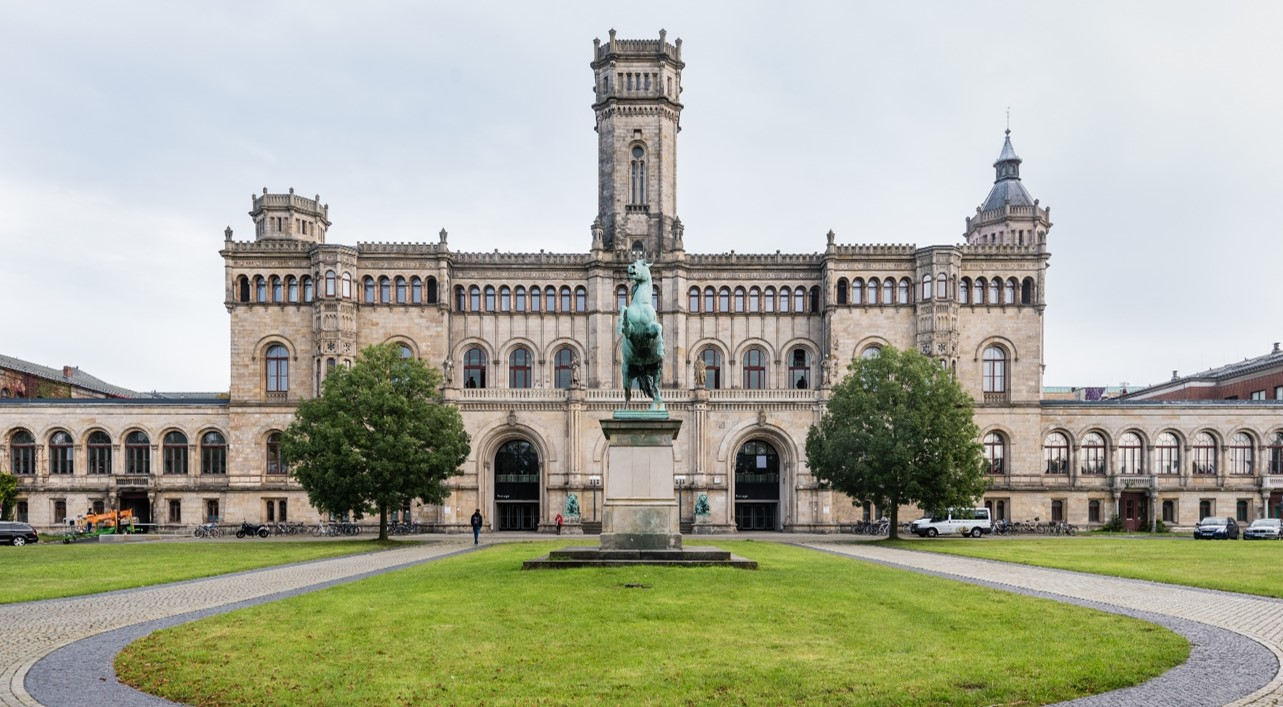
\includegraphics[width=0.65\textwidth]{figures/luh_default_presentation_title_image.jpg}}

% Title page: luhstyle
% \setbeamertemplate{title page}[luhstyle]
% % Add optional title image here
% \addtitlepageimage{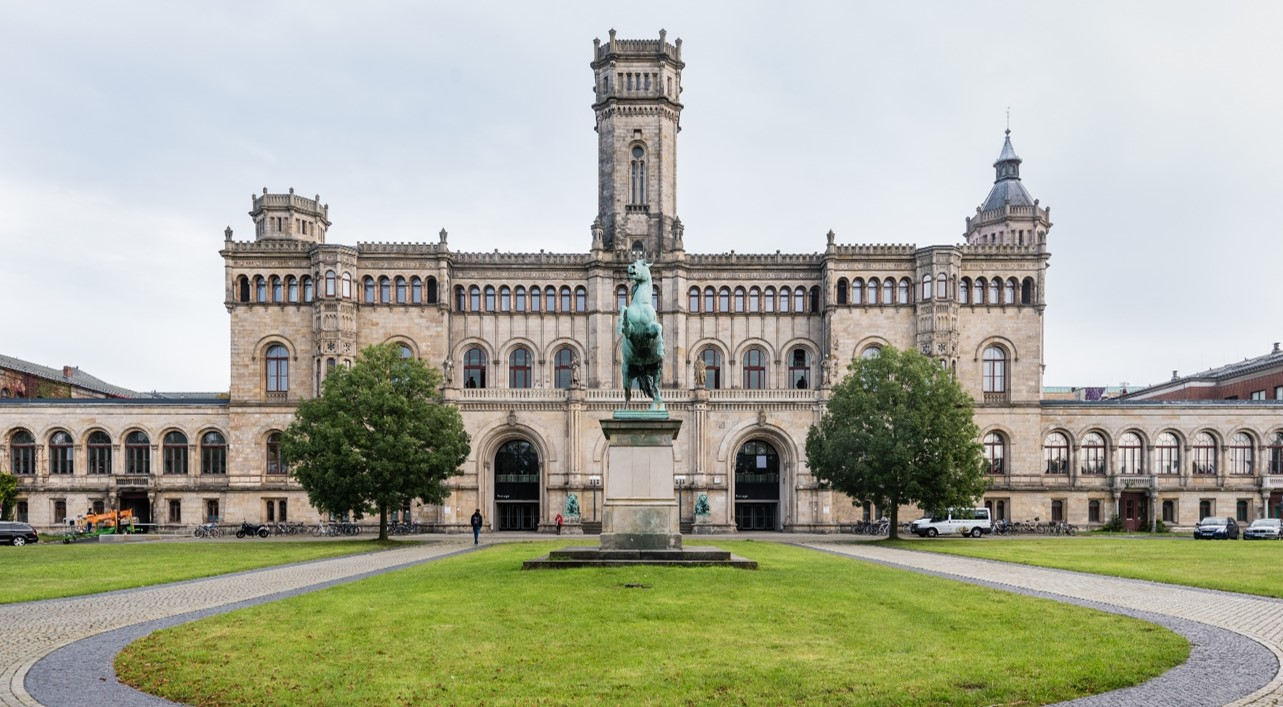
\includegraphics[width=0.75\textwidth]{figures/luh_default_presentation_title_image.jpg}}

\author[Abedjan \& Lindauer]{Ziawasch Abedjan \& Marius Lindauer\\[1em]
	
\includegraphics[height=\logoheight]{../latex_main/figures/luh_logo_rgb_0_80_155.pdf}\qquad
	
\includegraphics[height=\logoheight]{../latex_main/figures/DBIS_Kurzlogo.png}\qquad

\includegraphics[height=\logoheight]{../latex_main/figures/TNT_darkv4}\qquad

\includegraphics[height=\logoheight]{../latex_main/figures/L3S.jpg}	}
\date{Summer Term 2022; \hspace{0.5em} {
\includegraphics[height=1.5em]{../latex_main/figures/Cc-by-nc-sa_icon.svg.png}}; based on \href{https://ds100.org/fa21/}{[DS100]}
}


%%% Custom Packages
%----------------------------------------------------------------------
% Create dummy content
\usepackage{blindtext}

% Adds a frame with the current page layout. Just call \layout inside of a frame.
\usepackage{layout}


%%% Macros
%\renewcommand{\vec}[1]{\mathbf{#1}}
% \usepackage{bm}
%\let\vecb\bm

\title[Introduction]{DS: Principal Component Analysis}
\subtitle{Principal Component Analysis}

\graphicspath{ {./figure/} }
%\institute{}


\begin{document}
	
	\maketitle
	\begin{frame}{Principal Component Analysis}
	    What we just did was reduce 2-dimensional data down to a single dimension.
        There is a name for this procedure: principal component analysis (PCA)
        \begin{itemize}
            \item The “score vector” 	$Xv_1$	is called the first principal component (PC1) of X
            \item In reality, we can use PCA to calculate multiple scores, or multiple principal components
        \end{itemize}
        \bigskip
        Reasons to perform PCA:
        \begin{itemize}
            \item Create informative visualizations from high-dimensional data
            \item Remove dimensions that do not add much information (variance) to our data
            \item Use as a preprocessing algorithm for other learning algorithms (e.g. Logistic Regression)
            \item Use V matrix to determine which features contribute to the most important PCs
        \end{itemize}
	\end{frame}
	
	
	\begin{frame}{Multiple Scores}
	    In the previous example, we had 2-dimensional data (midterm exam and final exam), which we summarized by reducing down to one dimension.\\
	    However, we often start with many more dimensions, and capturing all of these features with just a single score for each individual isn’t a helpful summary. \\
	    But we can obtain multiple scores, by making use of the other rows in $V^T$. For example, if we wanted all d scores, we can do the following:
	    \begin{equation*}
	        XV = \left[\begin{array}{ccc}
	           \dots  &  x_1 & \dots \\
	           \dots  &  x_2 & \dots \\
	                  & \vdots & \\
	           \dots  & x_n  & \dots       
	        \end{array}\right]
	        \left[\begin{array}{cccc}
	           \vdots  &  \vdots &  &  \vdots \\
	           v_1     &  v_2    & \dots &  v_d \\
	           \vdots  & \vdots  &    & \vdots   
	        \end{array}\right] = \left[\begin{array}{cccc}
	           \vdots  &  \vdots &  &  \vdots \\
	           Xv_1     &  Xv_2    & \dots &  Xv_d \\
	           \vdots  & \vdots  &    & \vdots   
	        \end{array}\right]
	    \end{equation*}
	\end{frame}
	
	
	\begin{frame}{Multiple Scores}
	    Q: Would we ever want to use all d scores?\\
	    A: You might be tempted to use all d scores, but remember d is the number of features in the entire original dataset, so using all d scores would be counterproductive.\\
	    How to actually choose the number of scores to use will come later in the lecture.
	    \begin{equation*}
	        XV = \left[\begin{array}{ccc}
	           \dots  &  x_1 & \dots \\
	           \dots  &  x_2 & \dots \\
	                  & \vdots & \\
	           \dots  & x_n  & \dots       
	        \end{array}\right]
	        \left[\begin{array}{cccc}
	           \vdots  &  \vdots &  &  \vdots \\
	           v_1     &  v_2    & \dots &  v_d \\
	           \vdots  & \vdots  &    & \vdots   
	        \end{array}\right] = \left[\begin{array}{cccc}
	           \vdots  &  \vdots &  &  \vdots \\
	           Xv_1     &  Xv_2    & \dots &  Xv_d \\
	           \vdots  & \vdots  &    & \vdots   
	        \end{array}\right]
	    \end{equation*}
	\end{frame}
	
	
	
	\begin{frame}{PCA Procedure}
	    \begin{itemize}
	        \item[1]  Center (and often also standardize) your design matrix X.
	        \item[2] Compute the SVD of your new centered/standardized X: $X = U\Sigma V^T$
	    \end{itemize}
	    \begin{figure}
	        \centering
	        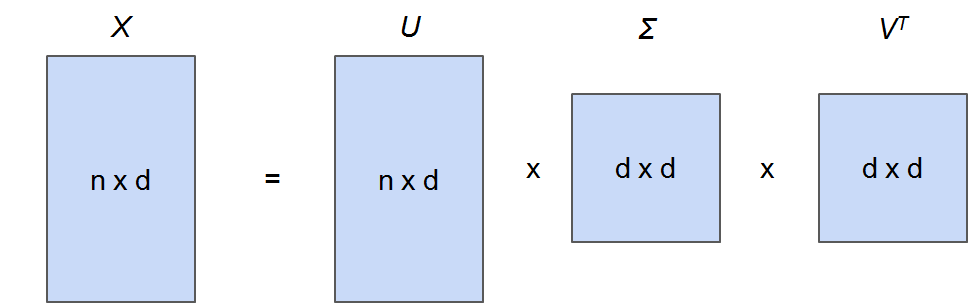
\includegraphics[scale=.5]{Bild12}
	    \end{figure}
	     \begin{itemize}
	        \item[1]  Compute all d principal components XV.
	        \item[2] Select the first ?? columns of XV as the principal components.
	    \end{itemize}
	\end{frame}
	
	
	\begin{frame}{Choosing Principal Components}
	    \begin{columns}
	        \begin{column}{.5\textwidth}
	                Goal: Capture as much information as possible, using as few principal components as possible.\\
	                How much information is in each principal component is encoded in the $\Sigma$ matrix, through the following relationship:
	                \begin{equation*}
	                    \sum\limits_{j=1}^d\sigma^2_j = n\sum\limits_{i=1}^dVar(X_i)
	                \end{equation*}
	                (You’ll explore this more in discussion.)
	        \end{column}
	        
	        
	        \begin{column}{.5\textwidth}
	            \begin{equation*}
	                \left[\begin{array}{cccc}
	                        \sigma_1 & 0 & \dots & 0 \\
	                         0 & \sigma_2 & \dots & 0 \\
	                        \vdots &     \vdots   &   \ddots  &  \vdots  \\
	                        0 & 0 & \dots &\sigma_d
	                    \end{array}\right]
	            \end{equation*}
	        \end{column}
	    \end{columns}
	\end{frame}
	
	
	\begin{frame}{Choosing Principal Components}
	    Goal: Capture as much information as possible, using as few principal components as possible.\\
	    We can capture all of the variance in our data by keeping all d principal components, but then we haven’t reduced our data at all. We can keep just one principal component, but then we might be losing a lot of variance.\\
	    Often, it is easier to talk about the fraction of total variance captured by a principal component, which is the following quantity:
	    \begin{equation*}
	        \frac{\sigma^2_i}{\sum_{j=1}^d\sigma^2_j} \hspace{.5cm}\underset{\leftarrow \text{n * Total Variance}}{} 
	    \end{equation*}
	\end{frame}
	
	
	\begin{frame}{Scree Plots}
	    We can plot the fraction of variance captured by each principal component in a scree plot:
	    \begin{figure}
	        \centering
	        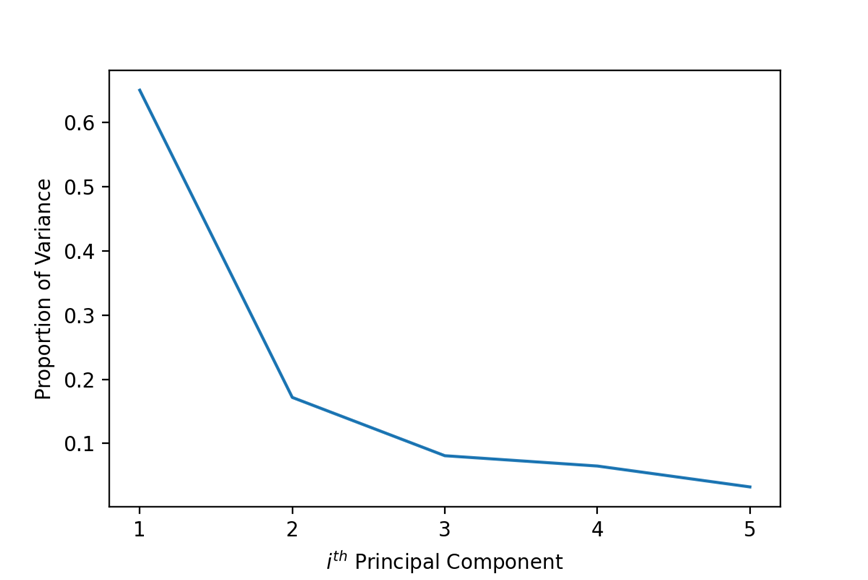
\includegraphics[scale=.5]{Bild13}
	    \end{figure}
	\end{frame}
	
	
	\begin{frame}{Scree Plots}
	 \begin{columns}
	     \begin{column}{.5\textwidth}
	         Each point tells us the proportion of total variance captured by the principal component.\\
	         Note that this plot is monotonically decreasing, this is because the σi are sorted!\\
	         To pick the number of PCs we want to use, we use the elbow method.\\
	         Note: There is no “right” answer, either 2 or 3 PCs would likely suffice here.
	     \end{column}
	     
	     
	     
	     \begin{column}{.5\textwidth}
	         \begin{figure}
	             \centering
	             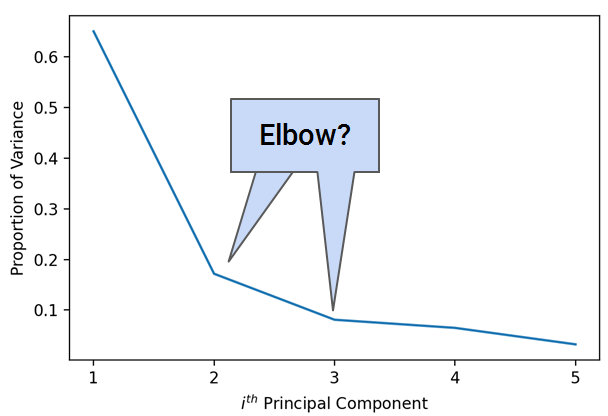
\includegraphics[scale=.45]{Bild14}
	         \end{figure}
	     \end{column}
	 \end{columns}
	    
	\end{frame}
	
	
	\begin{frame}{Interpreting $V^T$}
	 \begin{columns}
	     \begin{column}{.5\textwidth}
	         We know that the first row of $V^T$, $v_1$, is the direction that captures the most variance in our data.\\
	         \bigskip
	         We can use the $V^T$ matrix to determine which of our original features are more “important.”\\
	         \bigskip
	         Example: With the 2-column midterm and final dataset, the final was more important (larger weight in $V_1$)
	     \end{column}
	     
	     
	     
	     \begin{column}{.5\textwidth}
	        \begin{equation*}
	          v_1^T = [\begin{array}{cc}
	            0.573  & 0.820
	       \end{array}] 
	       \end{equation*}
	         \begin{figure}
	             \centering
	             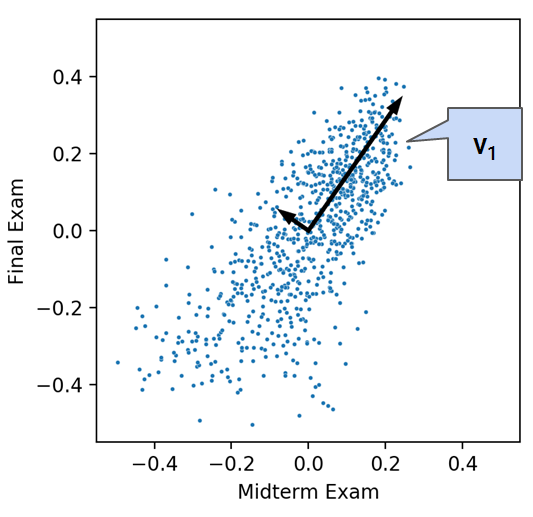
\includegraphics[scale=.35]{Bild15}
	         \end{figure}
	     \end{column}
	 \end{columns}
	    
	\end{frame}
	
	
	\begin{frame}{Interpreting $V^T$}
	    The magnitude of the numbers within each row of $V^T$ indicate how much the corresponding feature contributes to each principal component.
	    \begin{figure}
	        \centering
	        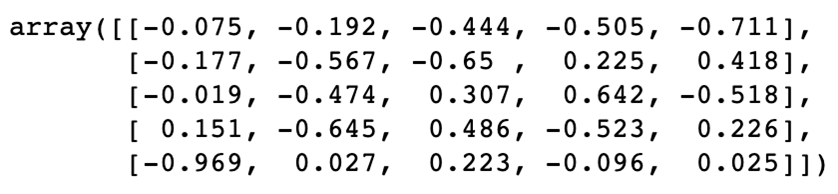
\includegraphics[scale=.5]{Bild16}
	    \end{figure}
	    
	    The last feature (final exam) contributes the most to PC1, so the final exam is a category that differentiates students well. \\
	    Note that the first feature (labs) doesn’t contribute much to the first 4 principal components, but dominates the last one—this is because most students receive the same score on labs.
	\end{frame}
	
	
	\begin{frame}{Interpreting the Principal Components}
	    \begin{columns}
	        \begin{column}{.5\textwidth}
	                We can also use the $V^T$ matrix to explain what our principal components actually mean.\\
	                PC1: Students who do above average in each of the different categories will have a more negative PC1. PC1 can be interpreted as a measure of overall success in the class.\\
	                \bigskip
	                PC2: Students with a large positive PC2 likely did well on the exams (midterm and final), but did badly on the other categories. The opposite is true for students with a negative PC2.\\
                    Generally, as you go “deeper” down, PCs lose interpretability.
	        \end{column}
	        
	        
	        \begin{column}{.5\textwidth}
	                \begin{figure}
	                    \centering
	                    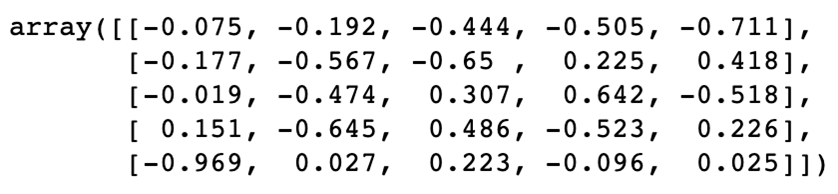
\includegraphics[scale=.4]{Bild16}
	                \end{figure}
	                
	                 \begin{figure}
	                    \centering
	                    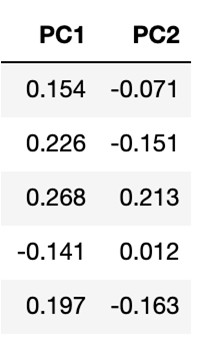
\includegraphics[scale=.5]{Bild17}
	                \end{figure}
	        \end{column}
	    \end{columns}
	    
	\end{frame}
\end{document}